\documentclass[9pt,twocolumn,twoside,lineno]{pnas-new}
% Use the lineno option to display guide line numbers if required.

\templatetype{pnasresearcharticle} % Choose template 
% {pnasresearcharticle} = Template for a two-column research article
% {pnasmathematics} %= Template for a one-column mathematics article
% {pnasinvited} %= Template for a PNAS invited submission

\title{The Geometry of Admixture}

% Use letters for affiliations, numbers to show equal authorship (if applicable) and to indicate the corresponding author
\author[a,1]{Benjamin M Peter}
%\author[b,1,2]{Author Two} 
%\author[a]{Author Three}

\affil[a]{Affiliation One}
%\affil[b]{Affiliation Two}
%\affil[c]{Affiliation Three}


\newcommand{\norm}[1]{\left\lVert #1 \right\rVert}
\newcommand{\nsq}[1]{\left\lVert #1 \right\rVert^2}



% Please give the surname of the lead author for the running footer
\leadauthor{Peter} 

% Please add here a significance statement to explain the relevance of your work
\significancestatement{Authors must submit a 120-word maximum statement about the significance of their research paper written at a level understandable to an undergraduate educated scientist outside their field of speciality. The primary goal of the Significance Statement is to explain the relevance of the work in broad context to a broad readership. The Significance Statement appears in the paper itself and is required for all research papers.}

% Please include corresponding author, author contribution and author declaration information
\authorcontributions{Please provide details of author contributions here.}
\authordeclaration{Please declare any conflict of interest here.}
%\equalauthors{\textsuperscript{1}A.O.(Author One) and A.T. (Author Two) %contributed equally to this work (remove if not applicable).}
\correspondingauthor{\textsuperscript{2}To whom correspondence should be addressed. E-mail: author.two\@email.com}

% Keywords are not mandatory, but authors are strongly encouraged to provide them. If provided, please include two to five keywords, separated by the pipe symbol, e.g:
\keywords{Principal component analysis $|$ admixture $|$ population structure $|$ geometry $|$ $F$-statistics $|$ ancientDNA}  

\begin{abstract}
Please provide an abstract of no more than 250 words in a single paragraph. Abstracts should explain to the general reader the major contributions of the article. References in the abstract must be cited in full within the abstract itself and cited in the text.
\end{abstract}

\dates{This manuscript was compiled on \today}
\doi{\url{www.pnas.org/cgi/doi/10.1073/pnas.XXXXXXXXXX}}

\begin{document}

\maketitle
\thispagestyle{firststyle}
\ifthenelse{\boolean{shortarticle}}{\ifthenelse{\boolean{singlecolumn}}{\abscontentformatted}{\abscontent}}{}

% If your first paragraph (i.e. with the \dropcap) contains a list environment (quote, quotation, theorem, definition, enumerate, itemize...), the line after the list may have some extra indentation. If this is the case, add \parshape=0 to the end of the list environment.
\dropcap{T}In the last decade, sequencing of thousands of ancient and modern human genomes has become feasible. In particular, ancient DNA extracted from bones has revolutionized our understanding of the prehistory of Eurasia and America,  with other continents likely to follow. 

With the increase in data also comes a challenge in interpreting the data; as gaps in samplings are filled and links between populations are established, paradigms relying on discrete populations become increasingly hard to apply, as hundreds of distinct units need to be joinly considered. 

As such, multivariate techniques such as principal component analysis (PCA) and Structure models are widely used to visualize human population structure, but usually they are not used to do inference directly.

Instead, one usually relies on an array of other approaches including the modelling of the SFS, PSMC-like approaches or admixture graphs; all of which have the issue that they can only handle a small number (typically less than 20) populations. Thus, complex inference typically relies on a combination of exploratory analyses, followed by a number of hypothesis tests investigating small subsets of the data. 

In human population genetics, a particularly fashionable choice are the F-statistics, that are used to test for admixture using 3 or 4 populations at a time. Typically, they are motivated by trees and admixture graphs, but they can be derived under arbitrary population genetic models (Peter, 2016).

However, establishing a connection between these two approaches remains difficult. 
Here, I present a connection between the exploratory PCA and the formal statistics. 

\subsection*{Model}
The $F$-statistics are defined as 
$$F_2(P_A, P_B) = E(p_a - p_b)(p_a - p_b)$$
$$F_3(P_A, P_B; P_X) = E(p_a - p_x)(p_b - p_x)$$
$$F_4(P_A, P_B, P_C, P_D) = E(p_a - p_b)(p_c - p_D)$$
where $P_i, p_i$ are populations and corresponding allele frequencies, respectively. Here, we think of the expectation over all loci in the genome.

Thus, for data from $n$ individuals and $L$ sites, a natural estimator for $F_3$ is
\begin{equation}
    F_3(A, B, X) = \frac{1}{L}\sum_i^L (p_{ai} - p_{xi})(p_{bi} - p_{xi}) - \hat{h}_x
\end{equation}
where $\hat{h}_x$ is an estimator of the heterozygosity.

Now, imagine we have a matrix $X$ containing all the data, and that all individuals are diploid so that $X_{ij} \in (0,1,2)$ Then, 

\begin{equation}
    F_3(A, B, X) = \frac{1}{2L}\sum_i^L (X_{ai} - X_{xi})(X_{bi} - X_{xi}) - \frac{1}{4}\sum_i X_{xi}(2-X_{xi}).
\end{equation}

Another common method to analyze population genetic data is PCA. Typically, \cite{mcvean2009} one constructs the row-normalized matrix $Y_i = X_i - \frac{1}{n}\sum_n X_i$, and performs a singular-value-decompositon, $X=UDV^T = UP$, where $P = DV^T$ is a $L \times n$ matrix of principal components, and $U$ is $L \times n$ matrix of loadings. 

As $(X_{ai}-X_{xi})(X_{bi}-X_{xi}) = (X_{ai}+\mu_i -X_{xi} - \mu_i)(X_{bi} + \mu_i-X_{xi}_i-\mu_i) = (Y_{ai}-Y_{xi})(Y_{bi}-Y_{xi})$, we can rewrite $F_3$ as

\begin{equation}
    F_3(A, B, X) = \frac{1}{2L}\sum_{k=1}^K (P_{ak}  - P_{xk})(P_{bk} - P_{xk}) - h_x.
\end{equation}

That is, with the exception of the bias-correction term $h_x$, the $F$-statistic can be split into terms corresponding to individual principal components.

One property of PCA is that the PCs are orthogonal and in decreasing order, and it is commonly observed in human population genetics that only a very small number of PCs contain biologically useful information. Hence, we can approximate the data by the first $K$ PCs. 


\subsection*{When is F3-negative?}
Given two samples $A$ and $B$, for which sample $X$ will we detect admixture?
As 
\begin{equation}
    2 F_3(A, B,X) = \nsq{A-X} + \nsq{B-X} - \nsq{A-B},
\end{equation}
it follows from the Pythagorean theorem that $F_3$ will be zero if  if $X$ lies on the $K$-dimensional sphere with diameter $$\norm{A,B}$, negative if it lies inside and positive outside (FIGURE). 

\subsection*{The geometry of $F_4$}
Given three samples $A, B$ and $C$, for which sample $X$ will $F_4$ be zero?
First, we characterize the space for which $F_4$ is zero:
\begin{equation}
    2 F_4(A, B | C, X) = \nsq{A-X} + \nsq{B-C} - \nsq{B-X} - \nsq{A-C} = 0,
\end{equation}

This equation is equivalent to the statement that the (skew-)quadrilateral spanned by the points (A, B, C and X) is orthodiagonal. Hence, $X$ lies in the plane that goes through the point $C$, and whose norm passes through $A$ and $B$. 

A special case is 
\begin{equation}
    2 F_4(A, B | A, X) =2 F_3(A, X | B) = \nsq{A-X} + \nsq{B-A} - \nsq{B-X},
\end{equation}
that arises when one considers the ``outgroup''-$F_3$-statistic or the question of which populations besides $A$ have contributed to an admixed population $X$. From the above, $F_3(A, X|B)$ is zero for samples on the plane passing through $X$ with norm perpendicular to the line passing through $A$ and $X$.

The further away $B$ is from the plane, the lower the $F_3$-statistic will be.

What can we say about $X, Y$ in
\begin{equation}
    2 F_4(A, B | X, Y) = \nsq{A-X} + \nsq{B-Y} - \nsq{A-Y} - \nsq{B-Y} = 0
    \text{?}
\end{equation}
$X, Y$ must lie on a plane perpendicular to the line segment $A-C$. 
What can we say about $X, Y$ in
\begin{equation}
    2 F_4(A, B | X, Y) = \nsq{A-X} + \nsq{B-Y} - \nsq{A-Y} - \nsq{B-Y} = k
    \text{?}
    \end{equation}
$X$ and $Y$ must lie on parallel planes with norm $A-C$ and a distance $k$ apart.

What can we say about $X, Y$ in
\begin{equation}
    2 F_4(A, X | C, Y) = \sum (A-X)(C-Y) = 0
    \text{?}
\end{equation}

As $$\sum(A-X)(C-Y) = \norm{A-X}\norm{C-Y}\cos{\theta} = 0,$$
it follows that the line segments AX and CY are orthognal. From this it follows that $X$ and $Y$ lie on orthogonal planes that pass through $A$ and $C$, respectively.




\subsubsection{F4-Ratio's in PC-space}
if we interpret $F_4(O,I,X,2)=k$ as a function of $X$, we obtain a plane that is i) orthogonal to OI and a distance of $k$ away from $P_2$. Thus, the $F_4$-statistics in the ratio
\begin{equation}
    \alpha = \frac{F_4(O,I,X,2)} {F_4(O,I,1,2)}
\end{equation}
corresponds to two parallel planes; and $\alpha$ measures the difference in distance to the plane through the point $P_2$.


\subsubsection{qpAdm}
Given a population $T$ of interest, and some outgroups (``right'' \textit{sensu} Patterson) populations $R_j$ and potential admixture sources (``left'') populations $S_i$, we aim to estimate the mixture coefficients $w_i$, s.t.

\begin{equation}
    \sum_i w_i F_4(T, S_i | R_1, R_2) = 0
\end{equation}
For fixed $T$, $R_1$, $R_2$, we know that the $F_4$ statistics lie on a plane orthogonal to $R_1, R_2$ and passing through $T$. Thus, we aim to find weights such that the weighted sum of the projection of $S_i$ onto that plane equals $T$. For more than two outgroups $R_j$, we generate a plane for each pair of populations from $R_j$, and jointly optimize in this space. This makes most sense if these planes are orthogonal to each other.



\section{Other bases}
\begin{enumerate}
    \item Treelet
    \item simple Trees
    \item Rotate for specific $F$-statistic
\end{enumerate}
\section{Spectral analysis of admixture statistics}
\begin{enumerate}
    \item Split $F$-statistics by basis vector
    \item Same $F$-stat may arise as different contributions
    \item can use clustering to infer shared history?
\end{enumerate}




\subsection*{Author Affiliations}

Max-Planck-Institute for Evolutionary Anthropology, Department of Genetics, 04103 Leipzig, Germany.

\subsection*{References}

%\begin{figure}%[tbhp]
%\centering
%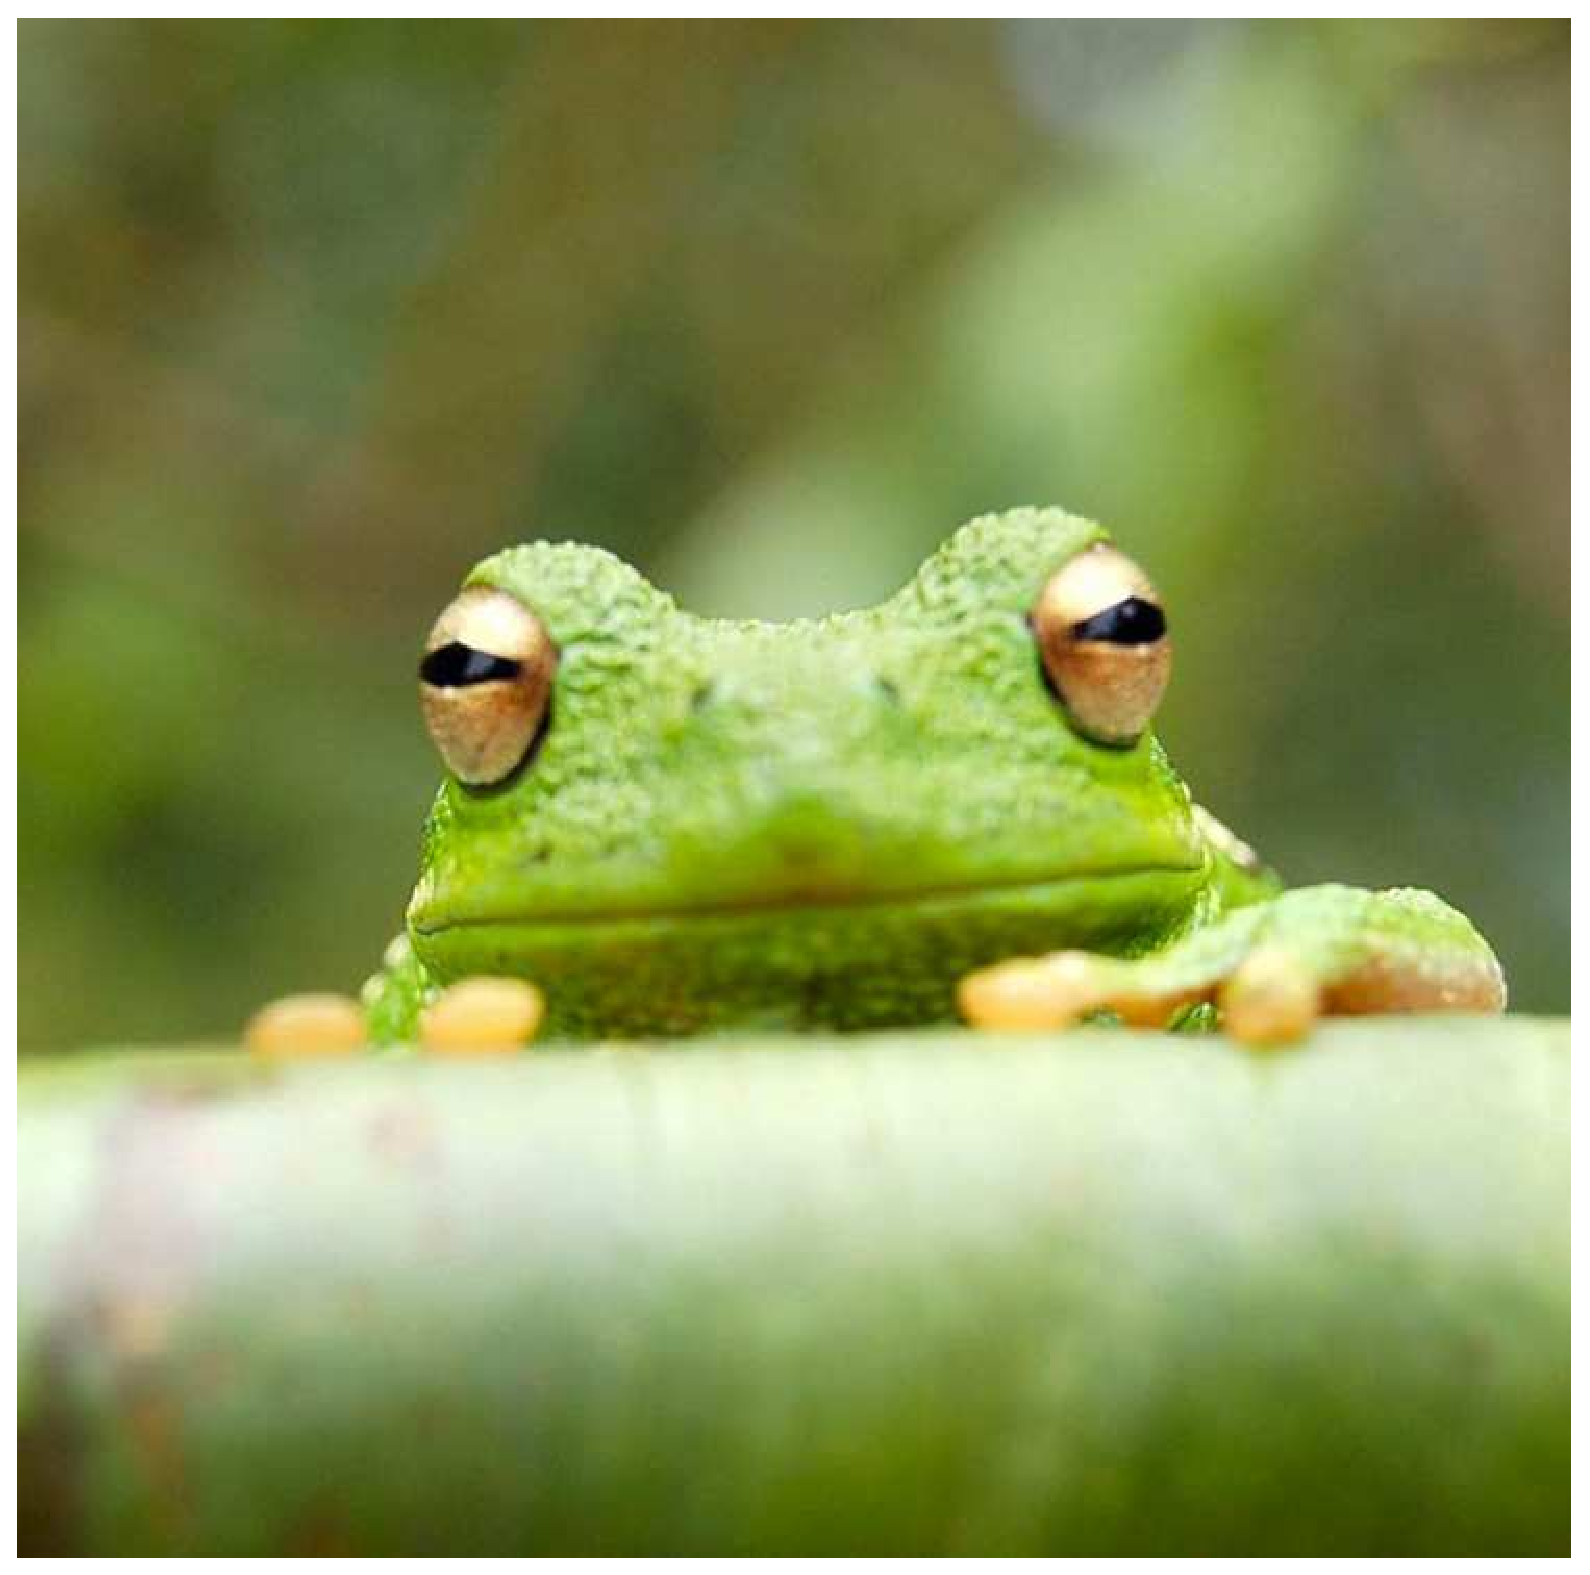
\includegraphics[width=.8\linewidth]{frog}
%\caption{Placeholder image of a frog with a long example caption to show %justification setting.}
%\label{fig:frog}
%\end{figure}


%\begin{SCfigure*}[\sidecaptionrelwidth][t]
%\centering
%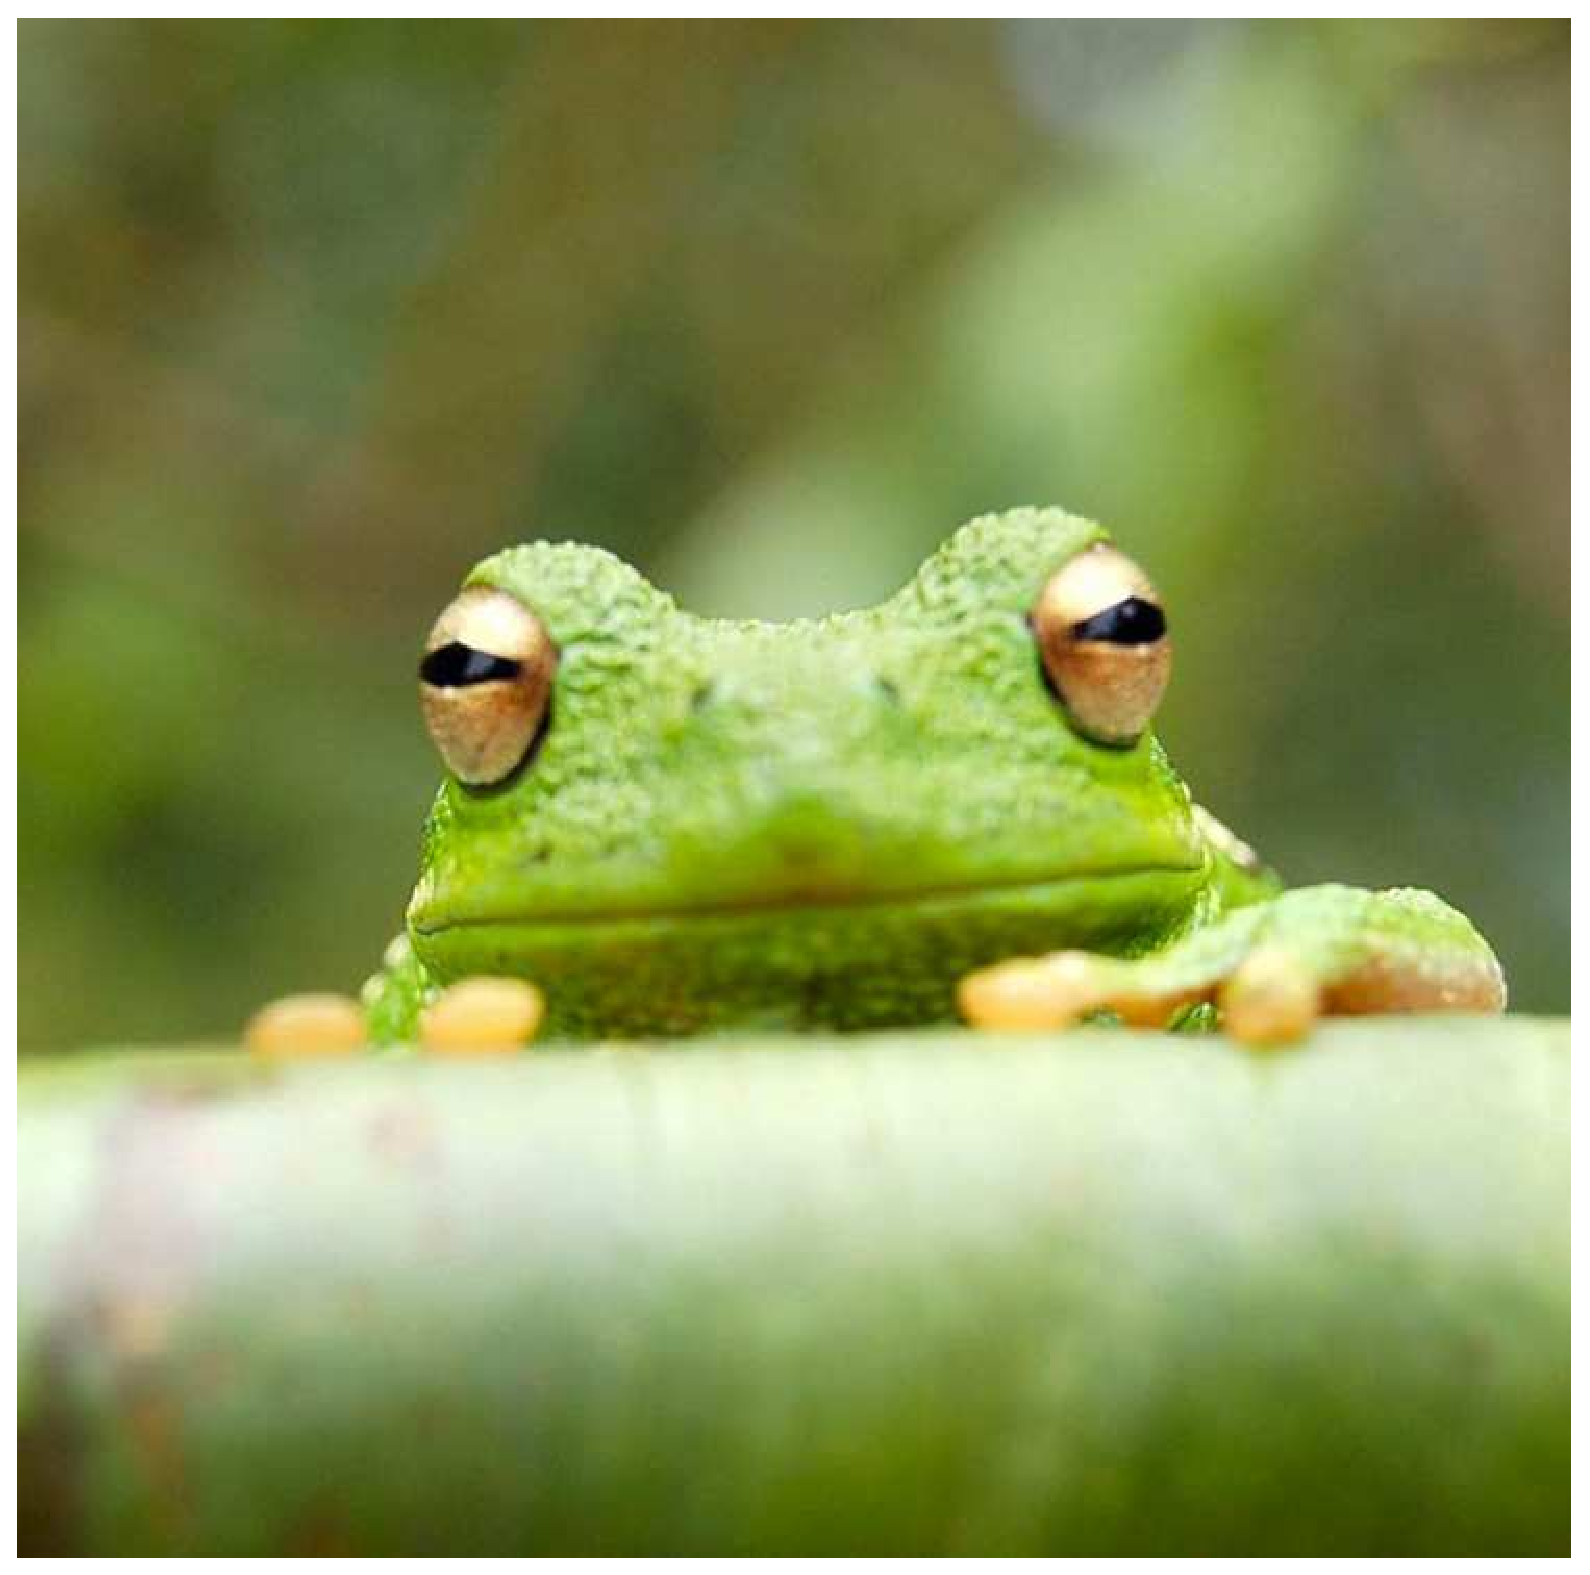
\includegraphics[width=11.4cm,height=11.4cm]{frog}
%\caption{This caption would be placed at the side of the figure, rather than %below it.}\label{fig:side}
%\end{SCfigure*}




\matmethods{
Let $A, B$ be populations; $L$ the number of loci and $a_l, b_l$ the number of 
derived alleles at locus $l$ when taking $n_l, m_l$ haploid individuals from populations $A$, $B$, respectively. Let $\mu_l$ be the mean allele frequency at locus $l$. The estimator for $F_2$ is 
\begin{eqnarray}
F_2(A,B) &= \sum_{l=1}^L (a_l-b_l)^2 - \frac{a_l (n_l - a_l)}{n_l^2(n_l-1)}- \frac{b_l (m_l - b_l)}{m_l^2(m_l-1)}
\end{eqnarray}

Furthermore, let $Q$ be an orthonormal basis on the space of loci, e.g. obtained through a PCA on the zero-centered data.  The square term
\begin{eqnarray}
S &=& \sum_{l=1}^L \big( (a_l - \mu_l) -(b_l -\mu_l)\big)^2\\
&=& \sum_{l=1}^L \big( \sum_k Q_{lk}P_{ka} - \sum_kQ_{lk}P_{kb}\big)^2\\
&=& \sum_{l=1}^L \left( \sum_k Q_{lk} (P_{ka} -P_{kb}) \right)^2\\
&=& \sum_{l=1}^L \left( \sum_k Q_{lk}^2 (P_{ka} -P_{kb})^2 + \sum_{k\neq k'} Q_{lk}Q_{lk'}(P_{ka} - P_{k'b})^2 \right)\\
&=& \sum_k\sum_{l=1}^L Q_{lk}^2 (P_{ka} -P_{kb})^2 + \sum_{k\neq k'}\sum_{l=1}^L Q_{lk}Q_{lk'} (P_{ka} - P_{k'b})^2\\
&=& \sum_k (P_{ka} - P_{kb})^2
\end{eqnarray}
The heterozygosity term, on the other hand, obeys
\begin{eqnarray}
H_a &=& \sum_{l=1}^L \frac{a_l (n_l - a_l)}{n_l^2(n_l-1)}\\
&=& \sum_{l=1}^L \frac{ (z_l + \mu_l) (n_l - (z_l + \mu_l))}{n_l^2(n_l-1)}\\
&=& \sum_{l=1}^L\frac{-z_l^2}{n_l^2(n_l-1)} + z_l \frac{n_l - 2\mu_l}{n_l^2(n_l-1)} + \frac{n_l\mu_l - \mu_l^2}{n_l^2(n_l-1)}\\
&\approx&  \sum_k \frac{-P_{ka}^2}{n^2(n-1)} + \sum_k P_{ka} \sum_l Q_{lk}\frac{n - 2\mu_l}{n^2(n-1)} + \sum_l\frac{n\mu_l - \mu_l^2}{n^2(n-1)}\\
&=&  -C_1 \sum_k P_{ka}^2 + \sum_k P_{ka} C_{2k}+ C_3
\end{eqnarray}
Without missing data, the constants $C_1= ({n^2(n-1)})^{-1}$; $C_{2k} =C_1\sum_l Q_{lk}(n - 2\mu_l)$ and $C_3= C_1\sum_l(n\mu_l - \mu_l^2)$ only depend on the sample size and $Q_{lk}$ and can be precomputed.




} 

\showmatmethods{} % Display the Materials and Methods section

\acknow{Please include your acknowledgments here, set in a single paragraph. Please do not include any acknowledgments in the Supporting Information, or anywhere else in the manuscript.}

%\showacknow{} % Display the acknowledgments section

% Bibliography
\bibliography{pnas-sample}

\end{document}